\chapter{State of the Art}
\label{chap:stateoftheart}

This chapter gives an overview of related research that has been done in the field of work
and aims to familiarize the reader with the subject. First, 
an overview of the legislation related to electromagnetic exposure and specific absorption rate
is given after which the related work about electromagnetic exposure is discussed.
The second section describes how UAV-networks are designed and how they can be optimized.
Finally, the used technologies are summed up including the type of drone, 
the characteristics of the cellular network and the type of antennae that are often used for this 
type of applications.

\section{Electromagnetic Exposure}

\subsection{Electromagnetic Field Radiation} % (fold)
\label{sub:emf}
People in wireless telecommunication networks are exposed to far-field electromagnetic radiation originating from base stations and other \gls{UE}. 
Network planners need to make sure
that the electromagnetic fields (expressed in V/m) do not exceed location dependent limitations enforced by the
government. 
These limits are location dependent. The \gls{EU} recommends the guidelines as defined by the \gls{ICNIRP} which limit electromagnetic exposure to 61 V/m.
Each European country needs to decide for themselves which limitations to enforce. Belgium for example delegated this responsibility to Flanders, Brussels and Wallonia \cite{J23}.
In order to have a comparable scenario, this study will be focused in the city center of Ghent. Therefore, the standards will be defined by the Flemish government, 
which state that in the 2.6 GHz frequency band, an individual antenna cannot exceed 4.5 V/m and the cumulative sum of all 
fixed sources has its maximum at 31 V/m \cite{J23, S13_normenBelgie}.

\subsection{Specific Absorption Rate}
The \gls{SAR} represents the rate at which electromagnetic energy is 
absorbed by human tissue with the thermal effect as its most important health consequence.
The volume of this tissue is typically 1 g ($SAR_{1g}$) or 10 g ($SAR_{10g}$). 
$SAR$ values can be categorized based on the covered area. As an example, 
the whole body \gls{SAR} ($SAR^{wb}$) is defined as the average radiation over the entire body while
localized \gls{SAR}-values only cover a certain part of the human body like the head.
The \gls{ICNIRP} has concluded that the threshold effect for $SAR^{wb}_{10g}$ is at 4 W/kg meaning that any higher absorption 
rate would overwhelm the \gls{thermoregulatory capacity} of the human body \cite{J23,J24}.
Whole body \gls{SAR}-values between 1 and 4 W/kg increase the temperature of the human body less than 1°C, which is proven not to be harmful 
for a healthy human being \cite{J24,P2}.
Thereafter, a safety factor of 50 for the public \cite{J23} is used to tackle unknown variables like experimental errors, increased sensitivity for certain population groups and so on. 
The \gls{EU} follows the recommendation from the \gls{ICNIRP} \cite{J23} and 
suggests a whole body $SAR_{10g}$ of 0.08 $W/kg$ and 2 $W/kg$ for localized $SAR_{10g}$ at head and torso area \cite{J31_bioeffects,J30}. 
The first metric is applicable for \gls{UE} and the second one for transmission towers \cite{S20}.
Belgium follows this recommendation \cite{J23,S13_normenBelgie}.
The \gls{FCC} of the \gls{USA} follows the recommendations of the \gls{IEEE} Std C95.1-1999 \cite{P1,P2} that defines 
regulations based on 1 g tissue.
The $SAR^{wb}_{1g}$ is therefore defined at 1.6 $W/kg$ despite the fact that this value has been reviewed and changed by the \gls{IEEE} to 8 $W/kg$ in Std C95.1-2005 \cite{P2}.
An overview is given in table \ref{table:overviewSARValues}.

%\begin{table}[h!]
%\begin{tabular}{|l|c|c|l|}
%\hline
%\textbf{Description} & \textbf{Value} & \textbf{Units} & \textbf{Institution}\\ \hline
%Max $SAR^{wb}_{10g}$                          &  $4$ & $W/kg$    & \gls{ICNIRP}     \cite{J23,J24}       \\ \hline
%Max $SAR^{wb}_{10g}$ for transmission towers               & $0.08$ & $W/kg$   & BE (\gls{EU})  \cite{J23,J31_bioeffects,J30,S20,J23,S13_normenBelgie}        \\ \hline
%Max $SAR_{10g}$ for \acs{UE} at head area                   & $2$ & $W/kg$    & BE (\gls{EU})     \cite{J23,J31_bioeffects,J30,S20,J23,S13_normenBelgie}    \\ \hline
%Max $SAR_{1g}$ for \acs{UE} at head area                 & $1.6$ & $W/kg$     &  \gls{USA} (\gls{FCC}, \gls{IEEE}) \cite{P1,P2}      \\ \hline
%\end{tabular}
%\caption{Overview of the different \acs{SAR} limitations.}
%\label{table:overviewSARValues}
%\end{table}

\begin{table}[h!]
\begin{tabular}{|l|c|c|}
\hline
\textbf{Institution}  & \textbf{Description} & \textbf{Value} & \textbf{Units} \\ \hline
\gls{ICNIRP}          & Max $SAR^{wb}_{10g}$                   &  $4$ & $W/kg$              \\ \hline
Belgium & Max $SAR^{wb}_{10g}$ for transmission towers                & $0.08$ & $W/kg$               \\ \hline
Belgium & Max $SAR_{10g}$ for \acs{UE} at head area (defined by the Belgian government)                  & $2$ & $W/kg$               \\ \hline
\gls{FCC} (\gls{USA} & Max $SAR_{1g}$ for \acs{UE} at head area                   & $1.6$ & $W/kg$               \\ \hline
\end{tabular}
\caption{Overview of the different \acs{SAR} limitations.}
\label{table:overviewSARValues}
\end{table}

The actual maximum \gls{SAR}-value of a phone is usually much lower. As an illustration, the 
iPhone 11 pro has a maximum $SAR_{10g}^{head}$ of 0.99 $W/kg$ \cite{S21} and a Samsung Galaxy S20 5G a
 $SAR_{10g}^{head}$ of 0.376 $W/Kg$ \cite{S22}. 
 %The phone with the highest recorded $SAR_{10g}^{head}$ value according to \cite{SARDatabase} is the discontinued LG 510W with a maximum of 1,94 $W/kg$.

\subsection{Related Work} % (fold)
\label{sub:general}
The goal of this master dissertation is the investigation of electromagnetic exposure considering all sources. Four types of sources are considered: the user's own phone,
 the base station that is serving this user, 
all devices from other users in the network and all 
other active base stations that are not serving this user. This electromagnetic radiation is thereafter
absorbed by the human body and will be expressed in \gls{SAR}-values. 
Any other type or source of electromagnetic radiation like bluetooth, WiFi or backhaul connections will not be considered.

Several papers calculate exposure originating from certain sources, but very  limited research has been done covering the whole picture.
Plets et al. addresses in \cite{J6_originalExposureFormula} the problem that electromagnetic exposure is often a neglected 
factor when designing a network. Therefore, they propose a heuristic indoor network planner aiming to optimize
exposure and coverage in a WiFi network. They conclude that higher allowed exposure limits and more separation between the user and 
the access point 
have positive influence on the throughput.
The authors of \cite{J1} used this knowledge 
to investigate electromagnetic exposure originating from base stations in a more outdoor environment
and propose a capacity based deployment tool capable of optimizing towards electromagnetic exposure and power consumption 
in order to support future green networks.
Plets et al. later extended their indoor network planner in \cite{J10_RDP} and \cite{J10.1} so that also  
\gls{UL} traffic from the user's device will be calculated. 
They did not only consider the electromagnetic radiation for \gls{UMTS} and WiFi
but also how much is absorbed by the body, which will be expressed as specific absorption rates. 
Since the authors only cover voice calls,
uplink SAR is expressed in localized SAR values while the downlink traffic is expressed in whole body SAR.
 With the advent of 5G, paper \cite{J17_kuehn2019modelling} has been 
published, describing a guideline on how the total exposure of in a hypothetical 5G network has to be modelled and applies it 
to various scenarios.
They discuss how localized SAR values are achieved from different sources including all mobile phones and all base stations.
They conclude that the user's own device is the most important contributor to the total localized SAR. 
The exposure for unconnected users is mainly originating from bystanders instead of base stations. The exposure 
from these bystanders will be four times higher than from base stations.
The authors also conclude that reducing the cell size has a positive influence on the exposure of active users by 
a factor 2 to 10.
In short, they state that a network with a lower path
loss, smaller cells and additional indoor coverage, helps to reduce total exposure.
Finally, Plets et al. published in \cite{J22_plets2015joint} how 
to minimize \gls{UL} and \gls{DL} exposure dose for an indoor environment. They describe how both \gls{UL} and \gls{DL} traffic 
can be converted in whole body SAR values making it possible to achieve an overall picture.
They conclude that a dose reduction of 75\% can be achieved by increasing number of base stations and decreasing transmission power.
Further, their optimization algorithm is able to reduce downlink doses for WiFi with more than
95\%. The reduction for \gls{UMTS} will vary between 73\% and 83\% and 
 the dose reductions for  \gls{LTE}  will be at least 80\%.
Thanks to power control, \gls{UMTS} and \gls{LTE} require an almost continuous uplink usage in order to 
see a significant effect by the optimization algorithm.

Research about \gls{SAR}-values have not only been done in function of an entire network. Also various papers 
exist considering other scenarios. In this way,
Mahfouz et al. performs an analysis on the total \gls{SAR} from a mobile phone considering the fact that the device contains multiple antennae. They
concluded that the localized \gls{SAR} for the different configurations never exceeds the limit defined by the \gls{ICNIRP} \cite{P3}.
The authors of \cite{P5} performed a research on the \gls{SAR}-values for the head area when the mobile phone is positioned in the near-field and 
far-field and concluded that a difference in \gls{SAR}-values was measured between both scenarios.  In \cite{P7} are the standardization efforts discussed
 to predict localized and whole body \gls{SAR} of users in and around the car when an antenna is attached to the outside of the car.
 Piuzzi et al. investigates in \cite{P8} the \gls{SAR} of numeric models. The model of the children is achieved by anatomically downscaling the adult.
 The results show that the whole body \gls{SAR} is higher for the children and therefore conclude that while the \gls{SAR} measured for an adult 
 might comply with restrictions enforced by the government, it is not necessarily the case for children. In \cite{P10} is the problem raised 
 that developing a numeric model, often used for \gls{SAR} analysis, is a timely and costly process. Therefore, an equation is proposed to 
 estimate whole body \gls{SAR} when using a half-wave dipole. Further, it is important to note that 
 \gls{UE} is not necessarily a mobile phone. For example, the authors of \cite{P11} 
 investigated the exposure of a user to a nearby smart metre and concluded that \gls{SAR} was well bellow the guideline restrictions. 
 As last, the authors from \cite{J10.1.1} explained the duality between \gls{UE} and base stations and concluded that the exposure 
 from \gls{UE} will decrease when the received signal improves. They also noticed that the
 exposure from \gls{UABS}s in a \gls{GSM} network is below than from \gls{UE}. 
 However, this is not always the case. An \gls{UMTS} network will, thanks to power control,
 drastically reduce the exposure from \gls{UE} and will therefore sometimes even be equal to radiation from the base station.

In a realistic network, some users are calling while others are using other types of telecommunication services like browsing the web.
Therefore, all absorbed electromagnetic exposure should be expressed in whole body SAR while still covering all sources.

\section{Optimized UAV-aided networks}

A \gls{UAV} knows several applications. It was originally mainly used to support the military for surveillance and remote attacks without 
endangering pilots \cite{U12}. However, \gls{UAV}s have recently become more accessible by the general public due to decreasing costs. This 
allowed \gls{UAV}s to be researched for various applications.

When attaching an antenna to a \gls{UAV}, it can be used as a gateway for cellular communication for \gls{UE} on the ground.
Such a flying base station will be called a \gls{UABS}. 
This has several advantages like mobility and rapid deployment which is ideal for emergency situations or temporary events. Thanks to this mobility,  
\gls{UABS}s can easily be repositioned to satisfy certain requirements. A \gls{UAV}-aided network also brings some challenges with it like 
the limited weight of the payload and sparse power supply.

Kawamoto et al. introduced in \cite{U11} a WiFi network with the support of  \gls{UAV}s while considering resource allocation 
and antenna directivity. 
Gangula et al. illustrates in \cite{U10} how \gls{UAV}s can be  used as a relay for \gls{LTE}. 
If a terrestrial base station is in \gls{NLOS} with a user, a
\gls{UABS} can be used as a relay.
Zeng et al. proposes in  \cite{U12} a tutorial in 5G-and-beyond wireless systems where challenges like 
energy consumption, mobility and antenna direction are discussed. 
Deruyck et al. designed in \cite{J2} a capacity based deployment tool for UAV-aided emergency
networks for large-scale disaster scenarios where an ideal flying height of 100 m is suggested. This was expanded 
in \cite{U1} with a performance evaluation of the direct-link backhaul of this tool where a slightly lower 
flying height of 80 metres is recommended.

These \gls{UAV}-aided networks can be optimized towards certain goals.
Mozaffari et al. provides in \cite{U3} guidelines on how to optimize and analyse \gls{UAV}s equipped for 
wireless communication equipment. Issues like deployment, performance and power consumption are addressed.
A research area that has been excessively studied is the location solutions optimization problem.
For instance, \cite{U4} provides an algorithm that minimizes latency, \cite{U7,U9}  minimizes interference between \gls{UABS} and \cite{U8} minimizes the 
distance between \gls{UABS} and \gls{UE}. Other papers investigate trajectory optimization like in \cite{U7,U6}.
Further, \cite{U3,U5} discuss several implementation approaches on how optimization algorithms should be tackled by discussing options like 
heuristic algorithms, \gls{exact algorithm}s and machine learning. 

Optimizing the network towards electromagnetic exposure is rather limited. For a terrestrial network, using traditional base stations,
Deruyck et al. discusses in \cite{J1} how the network can be optimized towards either a minimal exposure or minimal power consumption of the entire network.
However, to the best of the author knowledge, no research has been done where a \gls{UABS}-network has been optimized towards electromagnetic exposure.

\section{Technologies}
\subsection{Type of Drone}
\label{sec:typeofdrone}

The type of \gls{UAV} will have a major impact on the network performance.
Two types of 
drones are considered in \cite{J2}: an off-the-shelf drone affordable by the general public and a more robust one. The results in \cite{J2}
show that the second type will require less drones to cover the same number of users and will last longer in the air. The research in this paper
will therefore be done with the usage of the second type. A technical overview of this drone is given in table \ref{table:dronespecs}.
\newline
\newline
\begin{table}[h!]
\centering
\begin{tabular}{|l|c|c|}
\hline
 Parameter          & Value      & Units   \\    \hline
 Carrier power      & 13.0 &A \\
 Average carrier speed           & 12.0 &m/s       \\ 
 Average carrier power usage    & 17.33& Ah      \\ 
 Carrier battery voltage        & 22.2 &V \\ \hline
\end{tabular}
\caption{Specifications of the used drone.}
\label{table:dronespecs}
\end{table}

\subsection{Long Term Evolution}
The tool makes use of \gls{LTE}, by the general public better known as 4G.  \gls{LTE} allows better \gls{UL} and \gls{DL} data speeds 
compared to its predecessors and is based on an all IP architecture. This technology can cover macrocells supporting cell sizes ranging from 5 km up to 100 km. 
Macrocell antennae are usually used by transmission towers along highways or on top of buildings. LTE supports however also smaller cells like
femtocells covering only a few hundred meters. These femtocell antennae are therefore more portable, require less energy and will not require a telecommunication operator because
of their simplicity \cite{J34}. Femtocell base stations are therefore used by the deployment tool.
Further, \gls{LTE} also supports both \gls{FDD} and \gls{TDD}.

\gls{FDD} makes simultaneous \gls{UL} and \gls{DL} traffic possible by assigning different frequencies within the same frequency range 
to both data streams. A small guard band is used between the \gls{UL} and \gls{DL} direction in order to prevent interference. An illustration 
is given in fig \ref{fig:FDD}.

\gls{TDD} allows  \gls{UL} and \gls{DL} traffic by splitting the time domain. Meaning that both traffic directions use the same frequency and therefore
alternately (in time) use the same frequency. A small time interval is used to prevent interference in case of a slightly bad timed synchronization as 
illustrated in fig. \ref{fig:TDD}

Since it is assumed in this master dissertation that the user is continuously exposed without interruption, 
\gls{FDD} will be used throughout this document.

\begin{figure}[!h]
  \centering
  \begin{minipage}[b]{0.45\textwidth}
      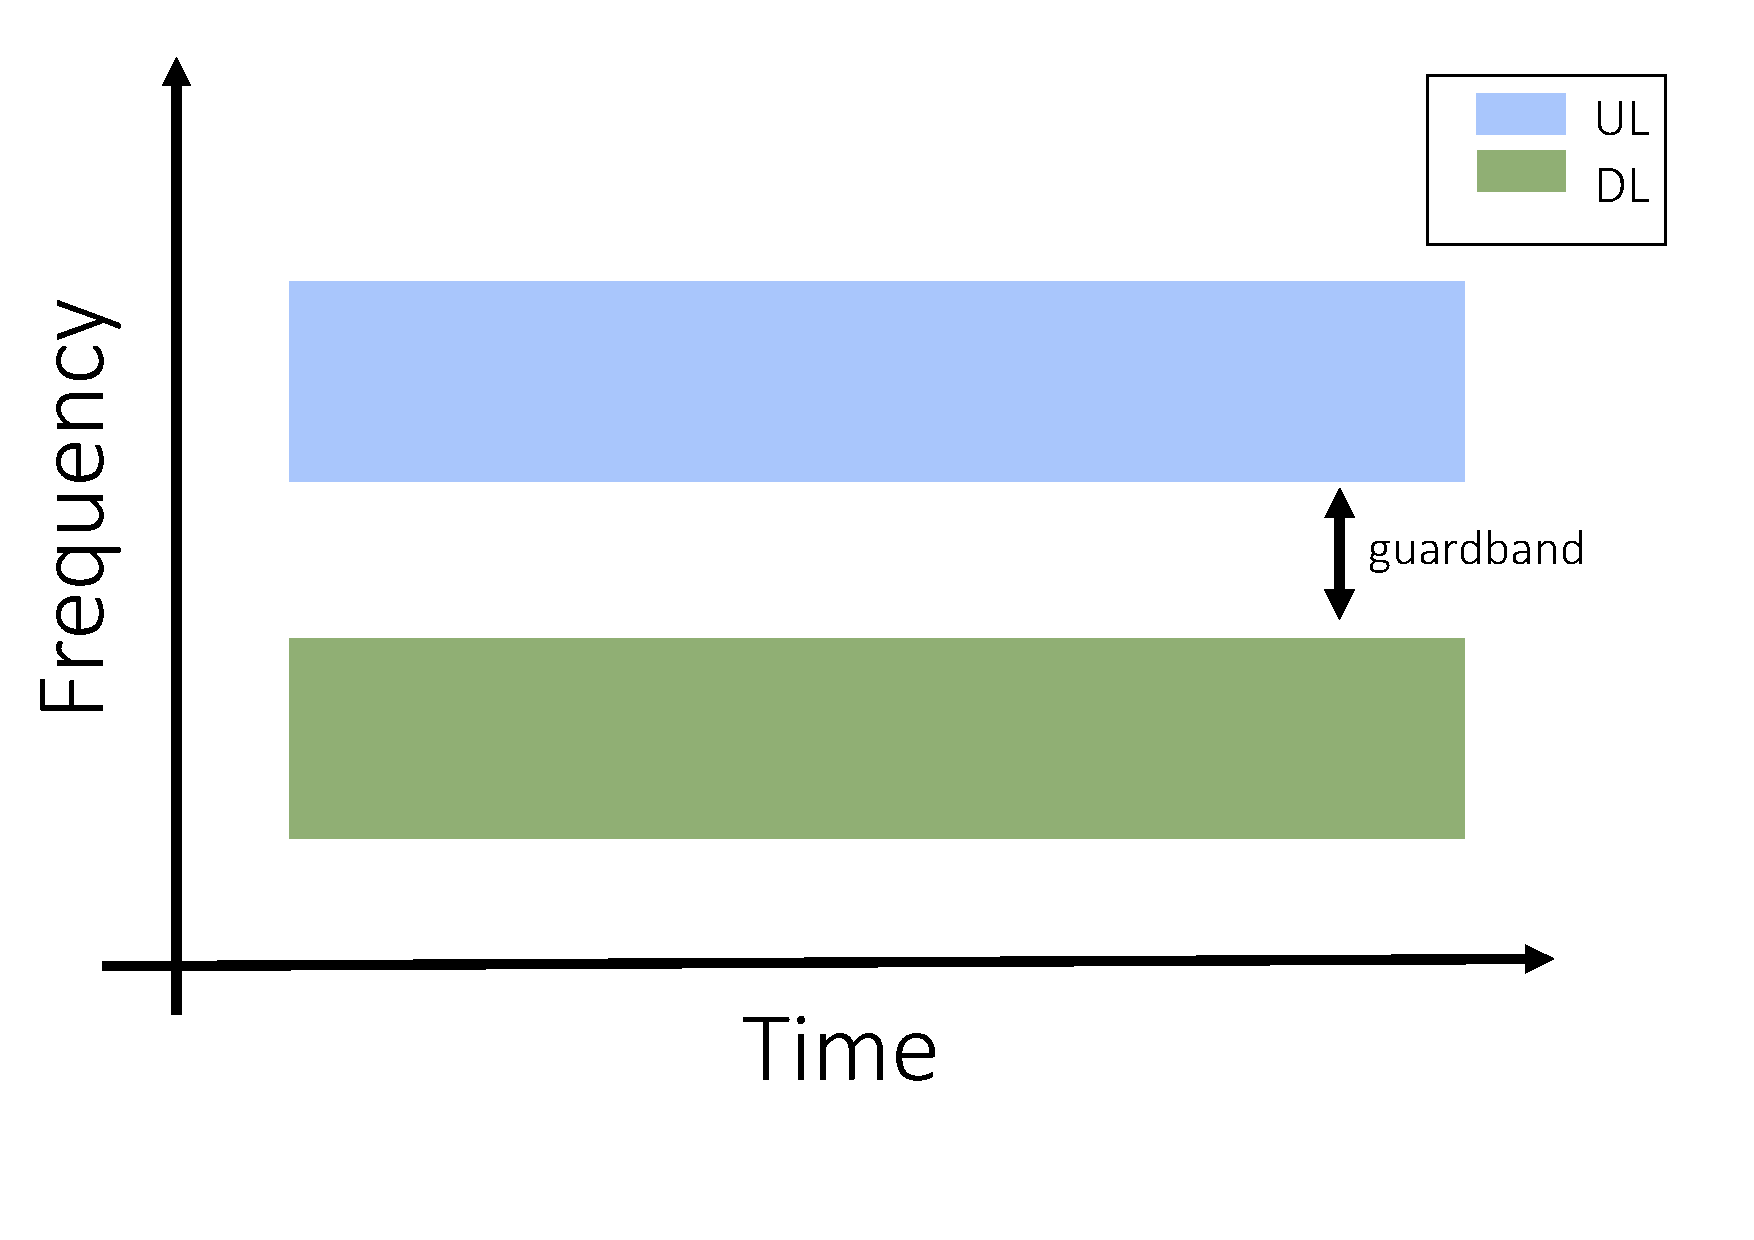
\includegraphics[width=\textwidth]{../images/FDDResourceAllocation.pdf}
    \caption{Resource allocation scheme for \acs{FDD}.}
    \label{fig:FDD}
  \end{minipage}
\hspace*{\fill}
  \begin{minipage}[b]{0.45\textwidth}
    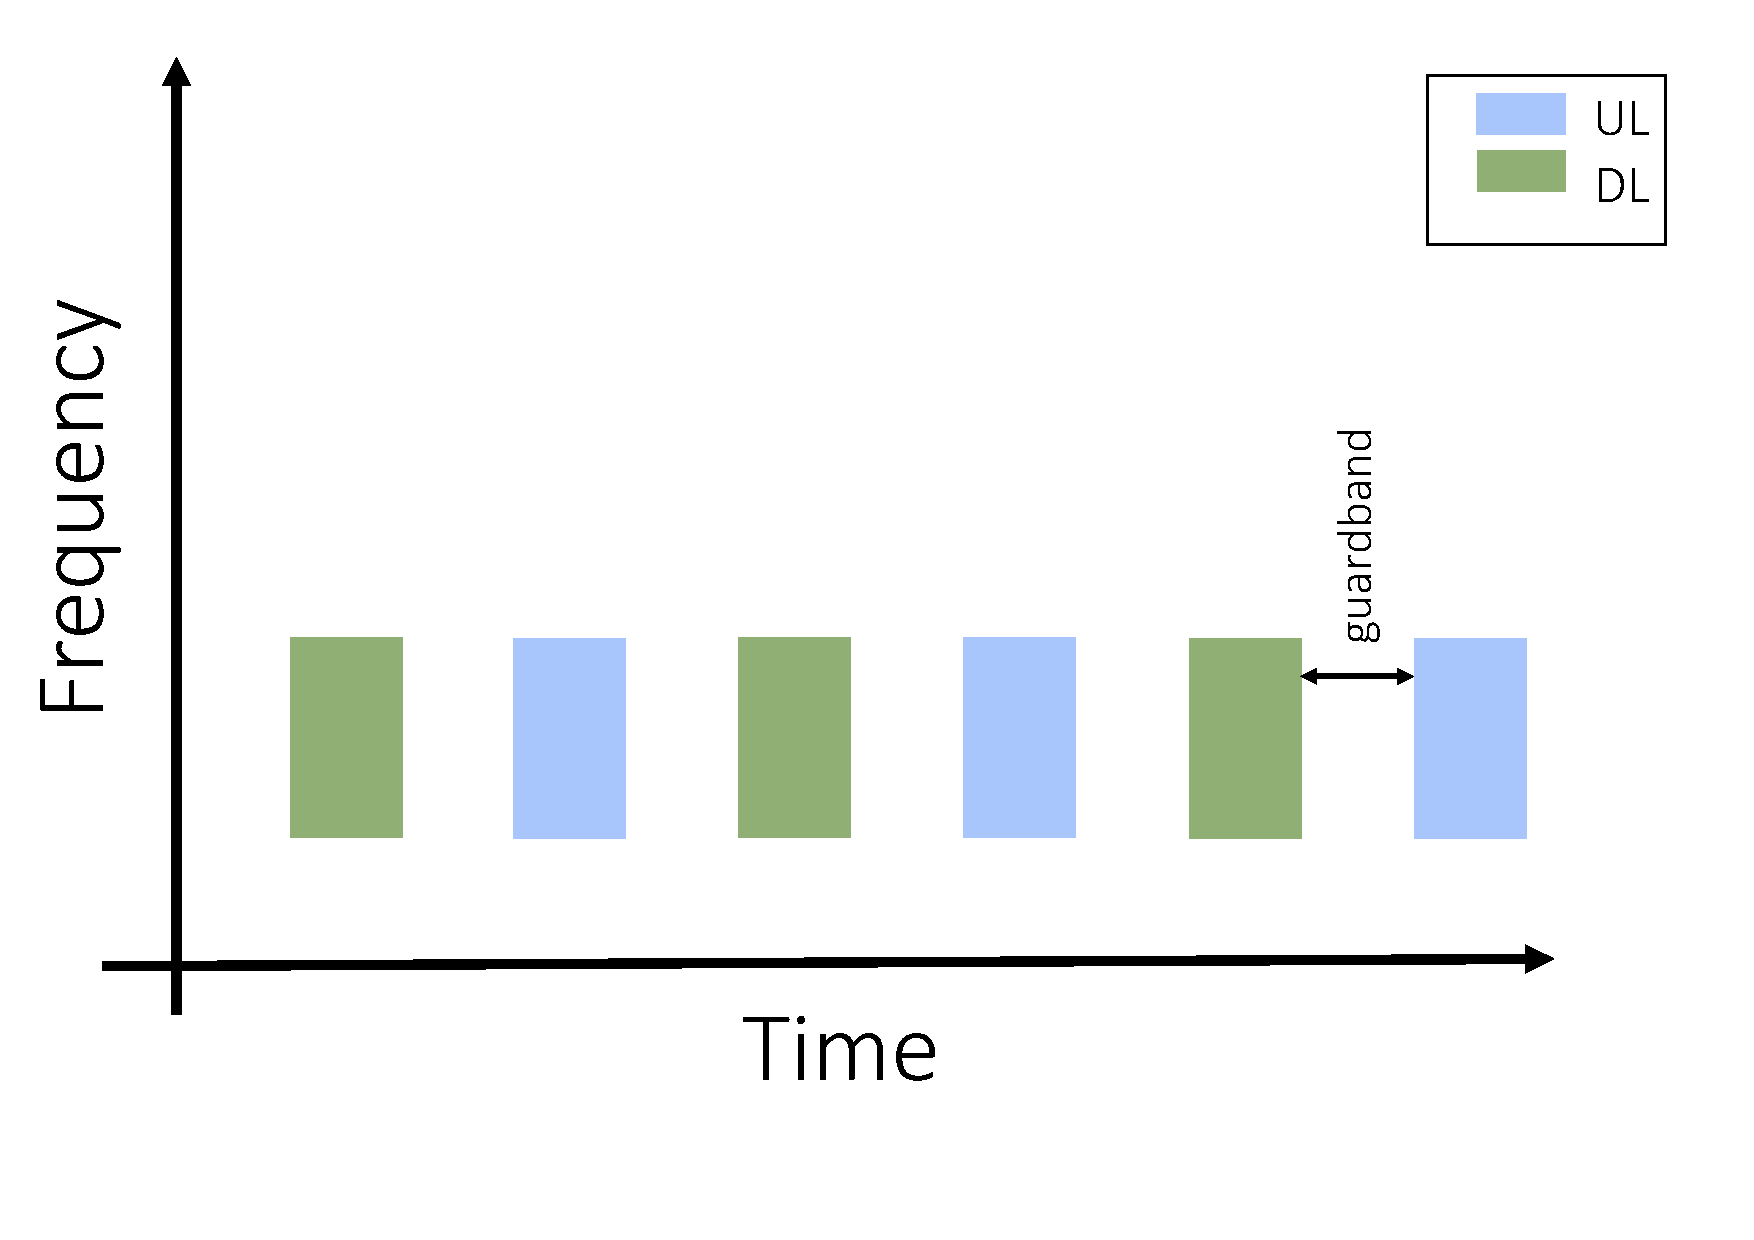
\includegraphics[width=\textwidth]{../images/TDDResourceAllocation.pdf}
    \caption{Resource allocation scheme for \acs{TDD}.}
    \label{fig:TDD}
  \end{minipage}
\end{figure}



\subsection{Type of Antennae} % (fold)

% problem antennae on drones
The onboard antenna of the \gls{UAV} will act as the gateway between the \gls{UE} and the backhaul network.
However, determining which antenna to use and how to position it, can be challenging.

Attaching an antenna to a \gls{UAV} brings some additional challenges with it as explained by Rizwan et al. in \cite{A1}.
Namely, the structure of the \gls{UAV} can influence the radiation pattern.  
This can either have a constructive or destructive impact and depends on the relative position between the \gls{UAV} and
the antenna.
When the antenna is too close to the \gls{UAV}, the \gls{UAV} can behave as a parasitic radiator, also emitting radiation.
When using a directional antenna, the influence of the \gls{UAV} will be much less but still existing, even when the \gls{UAV} is not 
positioned in the direction of the mean beam. \cite{A1} suggest that this side-effect can be reduced by introducing a little offset 
between the antenna and the \gls{UAV}.
Another challenge that comes with attaching an antenna to a \gls{UAV} is the need for 3D modelling of radiation patterns.
In traditional terrestrial networks,
the waves mainly propagated horizontally. When using \gls{UAV}s, waves will have to travel rather downwards 
causing 2D antenna modelling to become insufficient. A 3D-model which accounts for both elevation and azimuth directivity 
will be required \cite{U12}.

The easiest radiation pattern is a hypothetical  \gls{isotropicradiator} which radiates equally in all directions.
Antennae that radiate equal quantities for a certain plane  are called omnidirectional antennae \cite{U12} and several types 
exist.
Attaching a conventional dipole antenna array might be low-cost, yet they are too high in profile and weight \cite{A6}.
The authors of \cite{A9} and \cite{A11} both propose a broadband monopole blade antenna for \gls{UAV} applications 
but this type suffers from a large surface which is a big disadvantage for the limited space available on the used \gls{UAV}s in \ref{sec:typeofdrone}.
\cite{A10, A4} propose a broadband blade dipole antenna which is much smaller. Their wing-shaped design 
allows good aerodynamics when flying.
\cite{A12} proposes an alternative to blade 
antennae by presenting a wideband low profile monopole. The radiation pattern behaves similar to a traditional monopole but has 
a reduced height.
%meer bronnen en/of antennes voor bovenstaande paragraaf? Gebruik paragraaf 2 van de introductie uit https://ieeexplore.ieee.org/abstract/document/8357805

Another type of antennae are directional antennae that take advantage of throughput, lower interference and battery life \cite{A7}. This is done by focussing the 
electromagnetic energy there where it is needed.
One type of directional antennae that has been investigated excessively for \gls{UAV}-usage are microstrip antennae
since they provide several advantages compared to traditional antennae \cite{J13_microstripadvantages, J14_antennadesign}. Microstrip antennae
are lightweight, low in cost and thin causing them to be more aerodynamic which is a useful feature since the antennae will be attached
to \gls{UAV}s.
Zeng et al. proposes in \cite{A6} the use of such an antenna in a sunflower-shaped array configuration.
Also the authors from \cite{A5} attach star-shaped millimetre wave antennae to the wings of a \gls{UAV} and
\cite{A8} uses circular patch antennae in a circular array configuration for communication between \gls{UAV}s.

A basic microstrip antenna like the one presented in figure \ref{fig:basicpatchantenna} consists of a ground plane and
a radiating patch, both separated by a dielectric substrate. 
Several variations exist like microstrip patch antennae, microstrip slot antennae and printed dipole antennae which
all have similar characteristics \cite{J13_microstripadvantages, J14_antennadesign}. They are all thin, support dual frequency operation and they all have the disadvantage that they 
will transmit at frequencies outside the aimed band. This is also known as
\gls{spuriousradiation}. The microstrip patch and slot antenna support both linear
and circular polarization while the printed dipole only supports linear polarization. 
Further, the fabrication of a microstrip patch antenna is considered to be 
the easiest of the considered patch antennae \cite{J13_microstripadvantages}. 

\begin{figure}[H]
\centering
  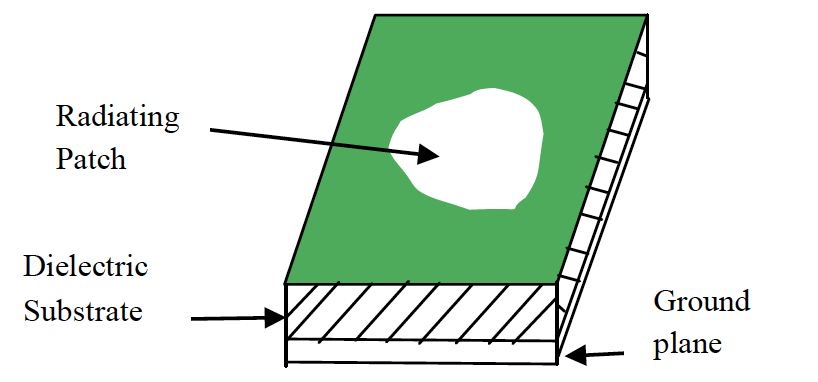
\includegraphics[width=\textwidth/2]{../images/patchantenna.png}
  \caption{General design of a microstrip antenna.}
  \label{fig:basicpatchantenna}
\end{figure}

The microstrip antenna requires besides the groundplane, dielectric substrate and the radiation patch also a feed line. Several feeding techniques exist of which the most popular are: coaxial probe feeding, microstrip line and aperture coupling. %and Microstrip Patch Antenna
%(todo: more refs? gebruik nummer twee van J13 (p2))

A first feeding method is the usage of a coaxial cable where the outer conductor is attached to the ground plane and the inner conductor to the radiations patch. Modelling is however difficult, especially for thick substrates as will be used in this master dissertation.
A second option is the usage of a microstrip line. This type of feeding is much easier to model since the microstrip line can be seen as en extension of the radiating patch.
A disadvantage is the increased \gls{spuriousradiation} which limits bandwidth.
A third is proximity coupling which has the largest bandwidth and low \gls{spuriousradiation}. It consists however of two dielectric substrates causing the overall thickness
of the antenna to increase as well as its fabrication difficulty \cite{J13_microstripadvantages}.
%(todo: tekst te weinig, bespreek ook apperture coupled attenna (zelfde paper als de rest))

The increasing usage of the microstrip patch antennae can be explained by its easy fabrication and lightweightness 
and therefore knows a widespread application in the millitary, global possitioning systems, telemedicine, 
WiMAX applications and so on.
The authors of \cite{J13_microstripadvantages} also state that some of the disadvantages like lower gain and power 
handling can be solved by using an array configuration.

The radiating patch is usually made of a thin layer of either gold or copper \cite{J14_antennadesign,J15_antennadesign}
and can have any form. However, shapes other than circles or rectangles would require large numerical computation \cite{J14_antennadesign}.
Thus, a simple rectangular shape will be used.
Further, also the \gls{dielectric constant} of the substrate is important. It typically varies between 2.2 and 12.
Finding a good dielectric depends on how the antenna will used. A lower
\gls{dielectric constant} with a thick substrate will result in better performance, better efficiency and larger bandwidths  \cite{J15_antennadesign}.
On the other hand, a larger \gls{dielectric constant} reduces de dimensions of the antenna \cite{J14_antennadesign}
which is also useful when attaching the 
antenna to a limited surface. Glass as a dielectric substrate with a constant of 4.4 will be used.

Figure \ref{fig:exampleDrone} shows a microstrip patch antenna 
constructed out of an aluminium patch and a teflon substrate. The microstrip patch 
antenna is pointing towards the ground since the \gls{UAV} will be flying above the user.

\begin{figure}[H]
\centering
  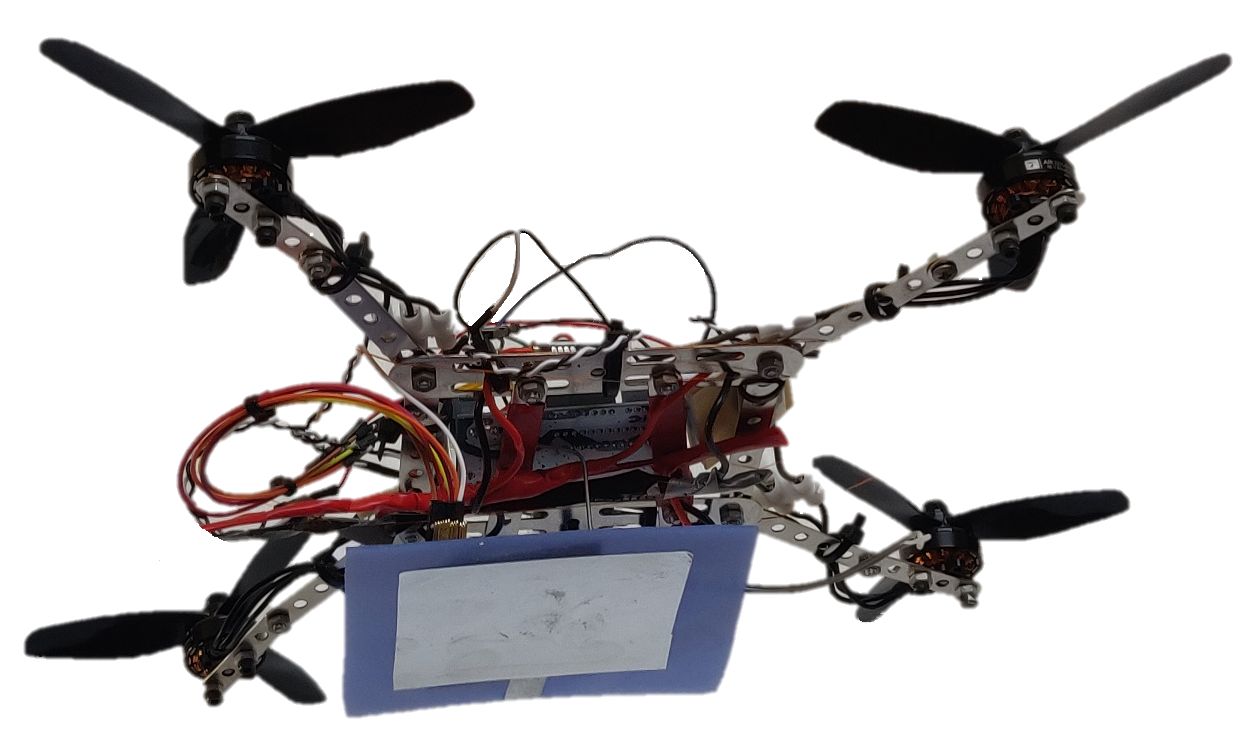
\includegraphics[width=0.8\textwidth]{../images/drone.png}
  \caption{Image of a microstrip patch antenna attached to the bottom of a \gls{UAV}. }
  \label{fig:exampleDrone}
\end{figure}


\section{Summary}
In this chapter, related papers are discussed that perform research in the same field as well
as the restrictions and guidelines by different organizations.
First, legislations about electromagnetic exposure and specific absorption rates are discussed followed 
by giving an overview of related work. The whole body \gls{SAR} from transmission towers in Belgium is limited to $0.08 W/kg$. It turns out a lot of research has been performed about electromagnetic exposure
but calculating whole body \gls{SAR} considering all \gls{UE} and all base stations is rather scarce.
Secondly, related work about \gls{UAV}-aided networks is presented. Various optimization strategies 
have been proposed in the past, including optimizing terrestrial networks towards electromagnetic radiation and power consumption. 
To the best of the author's knowledge, 
 exposure and power consumption optimized for a \gls{UAV}-aided networks remains unknown.

